Das grundlegende Problem, welches im Folgenden betrachtet wird, ist die unstrukturierte Suche. 
Es soll ein gegebenes Datum aus einer Menge von Datensätzen gefunden werden. 
Die Datensätze sind dabei entweder gänzlich unsortiert oder nach einem Kriterium, welches für die Suche keine Relevanz besitzt. 
Die Suche kann mit einer Funktion $\mathbf{f(x)}$ abgebildet werden, welche die Datensätze $\mathbf{x}$ als Eingabe akzeptiert. 
Der gesuchte Datensatz wird mit $\mathbf{\hat x}$ bezeichnet. Ist der Datensatz $\mathbf{x}$ nicht der Gesuchte, so gilt $\mathbf{f(x) = 0}$, andernfalls $\mathbf{f(\hat x) = 1}$. 
Die Datensätze sind dabei Teil der Menge $\mathbf{N}$ mit $\mathbf{N = 2^n}$. Die Suche ist dann erfolgreich, wenn ein Element $\mathbf{\hat x}$ gefunden wurde, für das $\mathbf{f(\hat x) = 1}$ gilt.
\newline
\\
Wird die Suche auf einem klassischen Rechner ausgeführt, so müsste dieser im schlechtesten Fall $\mathbf{f(x)}$ $\mathbf{N}$-mal auswerten. 
In diesem Fall wäre das gesuchte Element genau das letzte, welches aus der Menge $\mathbf{N}$ betrachtet wird. 
Dieser Fall ist jedoch sehr unwahrscheinlich und ein klassischer Rechner wertet $\mathbf{f(x)}$ im Durchschnitt $\mathbf{\frac{N+1}{2}}$ -mal aus, bis er das gesuchte Element findet.
Diese Laufzeit lässt sich unter der Verwendung von einem Quantencomputer mit dem Grover-Algorithmus deutlich verbessern. 
Der Grovers-Algorithmus erreicht eine quadratische Beschleunigung der Suche, indem $\mathbf{f(x)}$ nur noch $\mathbf{\sqrt{N}}$-mal ausgewertet werden muss. 
\\
\Cref{fig:laufzeitAufgabenstellung} zeigt anschaulich den Vergleich zwischen der schlechtesten (rot) und durchschnittlichen (blau) erwarteten Laufzeit eines klassischen Rechners sowie der Ausblick auf die Laufzeit, die mit dem Grover Algorithmus (grün) erreicht werden kann. Wie genau der Grovers-Algorithmus diese Beschleunigung erreicht, wird in den folgenden Abschnitten ausführlich erläutert.

\begin{figure}
    \centering
	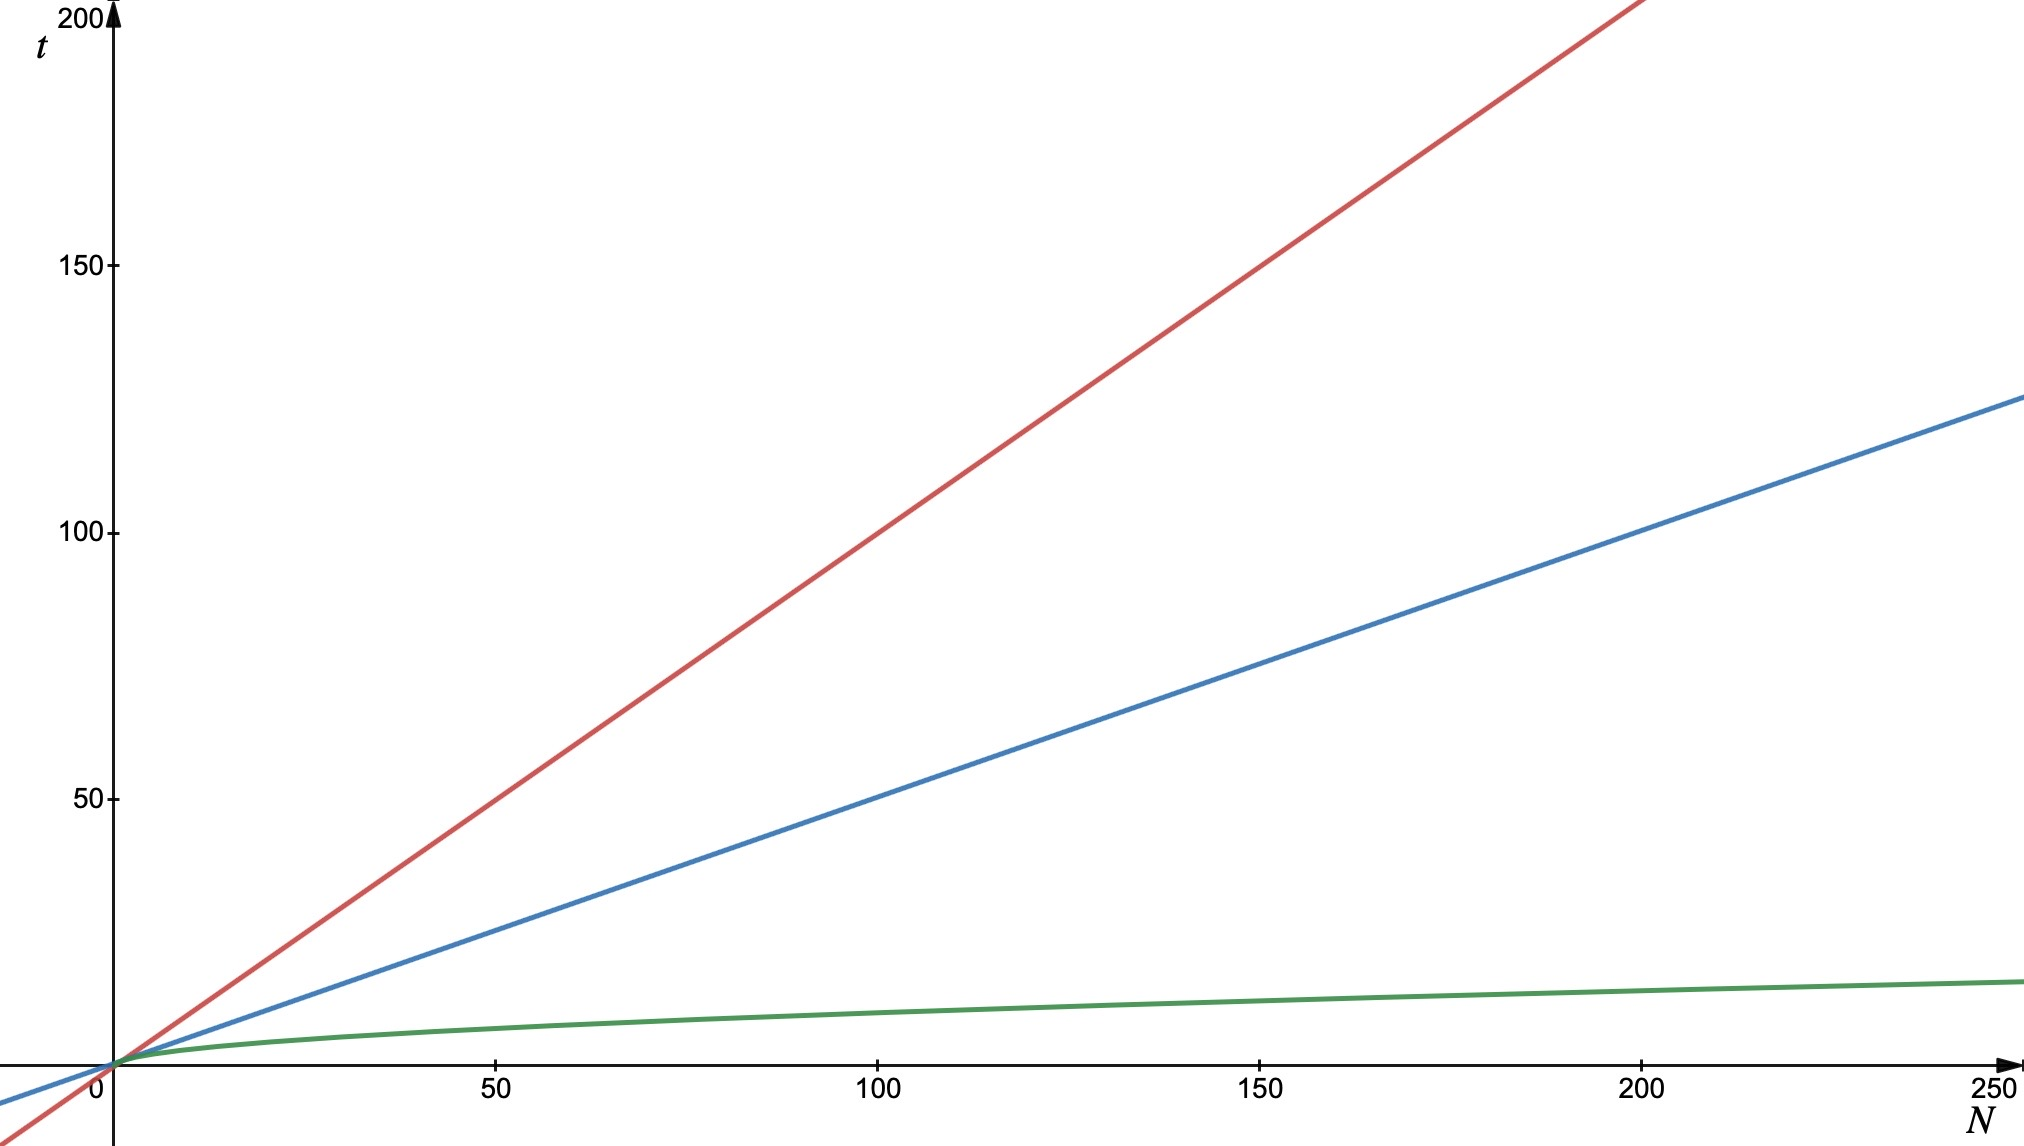
\includegraphics[width=0.7\textwidth]{figures/laufzeit-aufgabenstellung.jpg}
    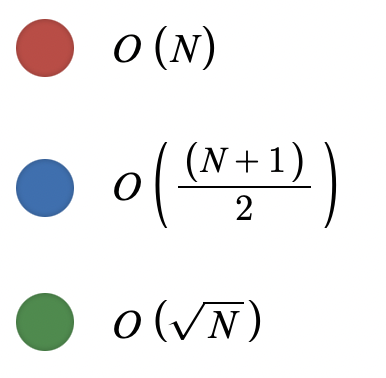
\includegraphics[width=0.165\textwidth]{figures/legende.png}

    \caption{Schlechteste (rot) und durchschnittliche (blau) erwartete Laufzeit einer Suche bei einem 
    \\klassischen Rechner sowie die Laufzeit des Grover Algorithmus (grün) 
    \\Quelle: Eigene Darstellung}

	\label{fig:laufzeitAufgabenstellung}
\end{figure}